\documentclass[12pt]{article}

\usepackage[german]{babel}
\usepackage{amsmath}
\usepackage{amssymb} % to display symbols for real numbers, integers etc. Usage: \mathbb{R}
\usepackage{graphicx}
\usepackage{listings} % to display programming code
%\usepackage[ngerman]{babel}
\usepackage{color}
\usepackage{relsize} % to display scaled math symbols (big summation symbol etc.)
\usepackage{textcomp}

\DeclareGraphicsExtensions{.pdf,.jpeg,.png}
\definecolor{listinggray}{gray}{0.9}
\definecolor{lbcolor}{rgb}{0.9,0.9,0.9}
\lstset{ % to display programming code in nice colors
	backgroundcolor=\color{lbcolor},
	tabsize=4,
	rulecolor=,
	language=matlab,
		basicstyle=\scriptsize, %for extra small font size
        upquote=true,
        aboveskip={1.5\baselineskip},
        columns=fixed,
        showstringspaces=false,
        extendedchars=true,
        breaklines=true,
        prebreak = \raisebox{0ex}[0ex][0ex]{\ensuremath{\hookleftarrow}},
		frame=single, %draw frame
        showtabs=false,
        showspaces=false,
        showstringspaces=false,
        identifierstyle=\ttfamily,
        keywordstyle=\color[rgb]{0,0,1},
        commentstyle=\color[rgb]{0.133,0.545,0.133},
        stringstyle=\color[rgb]{0.627,0.126,0.941},
        numbers=left,
        stepnumber=1,
        firstnumber=1,
        numberfirstline=true,
        linewidth=14cm,
}

\title{\"Ubungsblatt 9\\ \glqq Mustererkennung\grqq}
\author{J. Cavojska, N. Lehmann, R. Toudic}
\date{06.07.2015}
\begin{document}
\maketitle
%\renewcommand{\contentsname}{Table of Contents}
\tableofcontents
\newpage

\section{Aufgabe 1a - Trainingsmenge vs. Validierungsmenge}

\subsection{Code}
\begin{lstlisting}[language=Matlab]
Data   = load('pendigits-training.txt');

% prepare data for network
LData1 = horzcat(Data(1:60,1:16)./100, Data(1:60,17));
AData1 = horzcat(Data(1:60,1:16)./100,ones(60,1));
Label1 = Data(1:60,17);

LData2 = horzcat(Data(61:90,1:16)./100, Data(61:90,17));
AData2 = horzcat(Data(61:90,1:16)./100,ones(30,1));
Label2 = Data(61:90,17);

% weights
W1 = ones(17,16)*(-0.5);
W2 = ones(17,10)*(-0.5);

% learning rate
alpha = 1;

% training
quadErrorTraining = 0;
quadErrorTesting = 0;
numIter = 0
while quadErrorTraining >= quadErrorTesting
    clc
    [quadErrorTraining,quadErrorTesting, quadErrorTesting - quadErrorTraining]
    numIter = numIter + 1
    
    % start training
    dW1 = zeros(16,17);
    dW2 = zeros(10,17);
    quadErrorTraining = 0;
    quadErrorTesting = 0;
    % start training batch
    for i = 1:60
        d = AData1(i,:);
        l = Label1(i,:);
        
        % forward pass - layer 1
        t1 = d * W1;
        out_layer1 = 1 ./ (1 + exp(-t1));
        
        % forward pass - layer 2
        t2 = [out_layer1, 1]*W2;
        out_layer2 = 1 ./ (1 + exp(-t2));
        
        % error calculation
        lv = zeros(1,10);
        for j = 1:10
            if l == j
                lv(1,j+1) = 1;
            end
        end
        error = (out_layer2 - lv);
        quadErrorTraining = quadErrorTraining + 0.5*(error * error');
        
        % backward pass - layer 1        
        s1_der = out_layer1 .* (1 - out_layer1);
        D1 = diag(s1_der);

        % backward pass - layer 2
        s2_der = out_layer2 .* (1 - out_layer2);
        D2 = diag(s2_der);
        
        W2_                = W2(1:16,:);
        delta2             = D2*error';
        delta1             = D1*W2_*delta2;
        dW1                = dW1 + -alpha*delta1*d;
        dW2                = dW2 + -alpha*delta2*[out_layer1, 1];
    end
    W1                 = W1 + dW1';
    W2                 = W2 + dW2';
    
    
    % start testing
    
    for runs = 1:length(AData2)
        
        d     = AData2(runs,:);
        l     = Label2(runs);
            
        % forward pass
        % layer 1
        t1          = d * W1;
        out_layer1 = 1 ./ (1 + exp(-t1));
        
        % layer 2
        t2          = [out_layer1, 1]*W2;
        out_layer2 = 1 ./ (1 + exp(-t2));
        
        % error calculation
        lv = zeros(1,10);
        for j = 1:10
            if l == j
                lv(1,j+1) = 1;
            end
        end
        error = (out_layer2 - lv);
        quadErrorTesting = quadErrorTesting + 0.5*(error * error');
    end
end % end of while quadErrorTraining >= quadErrorTesting
\end{lstlisting}

\subsection{Resultate}
Unsere Loesung terminierte selbst nach mehreren Tagen und 30330600 Iterationen nicht. Sowohl der quadratische Fehler der Trainingsmenge als der der Validierungsmenge sinken beim Training, jedoch bleibt der quad. Fehler der Trainingsmenge immer groesser als der quad. Fehler der Validierungsmenge, wie der folgende Plot veranschaulicht:\\
\begin{center}
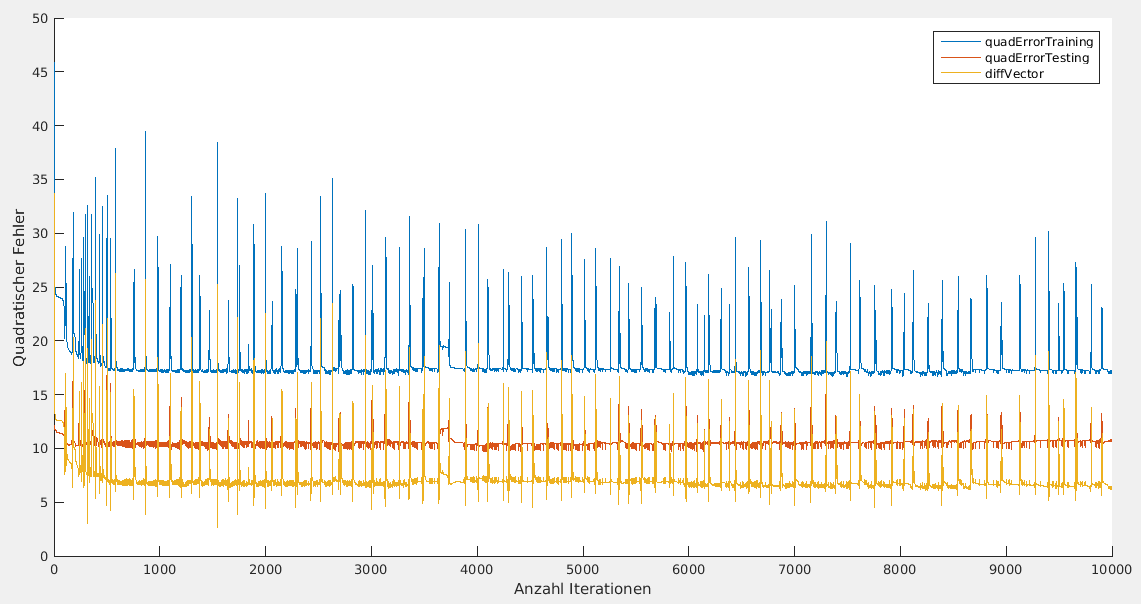
\includegraphics[width=13.5cm,height=10cm]{errorplot_aufg1a_10000_iter_quaddiff.png}
\end{center}
\newpage

\section{Aufgabe 1b - Rprop}
\subsection{Code}
\begin{lstlisting}[language=Matlab]
Data   = load('pendigits-training.txt');

% prepare data for network
LData1 = horzcat(Data(1:60,1:16)./100, Data(1:60,17));
AData1 = horzcat(Data(1:60,1:16)./100,ones(60,1));
Label1 = Data(1:60,17);

LData2 = horzcat(Data(61:90,1:16)./100, Data(61:90,17));
AData2 = horzcat(Data(61:90,1:16)./100,ones(30,1));
Label2 = Data(61:90,17);

% weights
disp('original weights:')
W1 = ones(17,16)*(-0.5);
W2 = ones(17,10)*(-0.5);

% Initialisierung der Rprop-Parameter
alpha = 0.0001; % learning rate
up = 1.5;
down = 0.2;
amax = 1;
amin = 0.01;
dE1_old = zeros(16,17);
dE2_old = zeros(10,17);
alphasdW1 = ones(16,17) * alpha;
alphasdW2 = ones(10,17) * alpha;

% training
quadErrorTraining = 0;
quadErrorTesting = 0;
numIter = 0

while quadErrorTraining >= quadErrorTesting
    clc
    numIter = numIter + 1
    disp('[quadErrorTraining, quadErrorTesting, difference]');
    [quadErrorTraining, quadErrorTesting, quadErrorTesting - quadErrorTraining]
    
    % start training
    dW1 = zeros(16,17);
    dW2 = zeros(10,17);
    quadErrorTraining = 0;
    quadErrorTesting = 0;
    dE1_acc = zeros(16,17);
    dE2_acc = zeros(10,17);
    for i = 1:60
        d = AData1(i,:);
        l = Label1(i,:);
        
        % forward pass - layer 1
        t1 = d * W1;
        out_layer1 = 1 ./ (1 + exp(-t1));
        
        % forward pass - layer 2
        t2 = [out_layer1, 1]*W2;
        out_layer2 = 1 ./ (1 + exp(-t2));
        
        % error calculation
        lv = zeros(1,10);
        for j = 1:10
            if l == j
                lv(1,j+1) = 1;
            end
        end
        error = (out_layer2 - lv);
        quadErrorTraining = quadErrorTraining + 0.5*(error * error');
        
        % backward pass - layer 1        
        s1_der = out_layer1 .* (1 - out_layer1);
        D1 = diag(s1_der);

        % backward pass - layer 2
        s2_der = out_layer2 .* (1 - out_layer2);
        D2 = diag(s2_der);
        
        W2_                = W2(1:16,:);
        delta2             = D2*error';      % 10x1
        delta1             = D1*W2_*delta2;  % 16x1
        dW1                = dW1 + -alphasdW1 .* sign(delta1*d);
        dW2                = dW2 + -alphasdW2 .* sign(delta2*[out_layer1, 1]);

        % accumulate error function gradient to use for backprop later:
        dE1_acc = dE1_acc + delta1*d;
        dE2_acc = dE2_acc + delta2*[out_layer1, 1];
    end % end of training batch
    W1                 = W1 + dW1';
    W2                 = W2 + dW2';
    
        
    % Lernraten mit Rprop anpassen:
    if numIter == 1
        dE1_old            = dE1_acc;
        dE2_old            = dE2_acc;
    else
        dE1                = dE1_acc; % Matrix der partiellen Ableitungen von E1 nach dem i-ten Gewicht sein
        dE2                = dE2_acc;
        dE1_new_old        = dE1 .* dE1_old;
        dE2_new_old        = dE2 .* dE2_old;
        dE1_old            = dE1;
        dE2_old            = dE2;
        
        % neue Lernraten fuer die Gewichte der 2. Schicht berechnen:
        for wi=1:size(dE2, 1)
            for wj=1:size(dE2, 2)
                if (dE2(wi, wj) * dE2_old(wi, wj)) > 0  % beschleunigen
                    alphasdW2(wi, wj) = min(alphasdW2(wi, wj) * up, amax);
                elseif (dE2(wi, wj) * dE2_old(wi, wj)) < 0  % bremsen
                    alphasdW2(wi, wj) = max(alphasdW2(wi, wj) * down, amin);
                end
            end
        end
        
        % neue Lernraten fuer die Gewichte der 1. Schicht berechnen:
        for wi=1:size(dE1, 1)
            for wj=1:size(dE1, 2)
                if dE1(wi, wj) * dE1_old(wi, wj) > 0  % beschleunigen
                    alphasdW1(wi, wj) = min(alphasdW1(wi, wj) * up, amax);
                elseif dE1(wi, wj) * dE1_old(wi, wj) < 0  % bremsen
                    alphasdW1(wi, wj) = max(alphasdW1(wi, wj) * down, amin);
                end
            end
        end
    end % end of rprop calculations
    
    
    
    % start testing
    
    for runs = 1:length(AData2)
        
        d     = AData2(runs,:);
        l     = Label2(runs);
            
        % forward pass
        t1          = d * W1;
        out_layer1 = 1 ./ (1 + exp(-t1));
        
        t2          = [out_layer1, 1]*W2;
        out_layer2 = 1 ./ (1 + exp(-t2));
        
        % error calculation
        lv = zeros(1,10);
        for j = 1:10
            if l == j
                lv(1,j+1) = 1;
            end
        end
        error = (out_layer2 - lv);
        quadErrorTesting = quadErrorTesting + 0.5*(error * error');
    end
end % end of while quadErrorTraining >= quadErrorTesting
\end{lstlisting}

\subsection{Resultate}
Diese auf der Aufg. 1a basierende Implementierung von Rprop terminiert leider auch nicht.

\end{document}